% 默认配方: xelatex -> biber -> xelatex -> xelatex
% 与 HW1/HW2 报告保持同一 elegantpaper 样式。
\ifdefined\ELEGANTBibTeXBackend
  \PassOptionsToClass{bibtex}{elegantpaper}
\fi

\documentclass[lang=cn,a4paper,newtx,nofont,code=minted]{elegantpaper}

% 避免 macOS 系统 CJK 字体在 XeLaTeX 中触发偶发 glyph 映射错误，固定使用 TeX Live 自带 Fandol 字体。
\setCJKmainfont{FandolSong-Regular.otf}[
  Path=/usr/local/texlive/2026/texmf-dist/fonts/opentype/public/fandol/,
  BoldFont=FandolSong-Bold.otf,
  ItalicFont=FandolKai-Regular.otf
]
\setCJKsansfont{FandolHei-Regular.otf}[
  Path=/usr/local/texlive/2026/texmf-dist/fonts/opentype/public/fandol/,
  BoldFont=FandolHei-Regular.otf
]
\setCJKmonofont{FandolFang-Regular.otf}[
  Path=/usr/local/texlive/2026/texmf-dist/fonts/opentype/public/fandol/
]

\usepackage{tabularx}
\usepackage{float}
\usepackage[section]{placeins}
\usepackage{array}
\usepackage{siunitx}
\usepackage{subcaption}
\usepackage{makecell}
\usepackage{enumitem}
\usepackage{xurl}
\graphicspath{{pic/}{../pic/}}

\renewcommand{\topfraction}{0.9}
\renewcommand{\textfraction}{0.07}
\renewcommand{\floatpagefraction}{0.8}
\setlength{\textfloatsep}{10pt plus 2pt minus 2pt}
\setlength{\floatsep}{8pt plus 2pt minus 2pt}
\setlength{\intextsep}{8pt plus 2pt minus 2pt}
\captionsetup[table]{font=small,labelfont=bf,skip=4pt}
\captionsetup[figure]{font=small,labelfont=bf,skip=3pt}
\setlength{\tabcolsep}{4pt}
\renewcommand{\arraystretch}{1.08}
\sisetup{detect-all,detect-weight=true,detect-family=true,group-digits=false,table-number-alignment=center,table-text-alignment=center}
\newcolumntype{L}[1]{>{\raggedright\arraybackslash}p{#1}}
\newcolumntype{C}[1]{>{\centering\arraybackslash}p{#1}}
\newcolumntype{R}[1]{>{\raggedleft\arraybackslash}p{#1}}
% code snippets are emitted as escaped 	exttt blocks.

\title{CS60003 期末作业实验报告：3DGS/AIGC 资产融合与 ACT 跨环境泛化}
\author{夏商周 \quad 25210980114 \quad Task1 多源资产生成、3DGS/AIGC 模型训练与资产导出 \\ 杨智超 \quad 25210980124 \quad Task1 统一表示、坐标对齐、融合渲染、相机与视觉优化、报告整合 \\ 杨晨 \quad 25210980120 \quad Task2 数据处理、ACT 训练、跨环境评估与统计分析}
\institute{\href{https://github.com/YangChen-pro/CS60003}{代码仓库}\quad|\quad\href{https://modelscope.cn/models/youngchen/CS60003/}{模型仓库}}
\date{\zhdate{2026/06/17}}

\begin{document}
\maketitle

\begin{abstract}
本报告对应 CS60003 期末作业。Task 1 完成了真实物体 3DGS 重建、文本到 3D 生成、单图到 3D 生成、Mip-NeRF 360 背景重建，以及统一 Gaussian splat 表达下的多源资产融合渲染。最终视频直接加载 A/background 的 3DGS splat 与 B/C 的纹理 Mesh surface splat，在同一 \texttt{gsplat} renderer 和前景聚焦相机轨迹下输出 1920$\times$1080、24 fps、6 秒漫游视频。Task 2 完成基于 LeRobot ACT 的 CALVIN 跨环境泛化实验：分别训练环境 A 单环境策略与环境 A/B/C 多环境联合策略，并在未见过的环境 D 上做 zero-shot 离线评估。主要结果使用不依赖 D 环境选模的 \texttt{final.pt}，多环境模型将 Action L1 从 0.1886211640 降至 0.1549013643，相对提升 17.88\%。配对统计显示，\texttt{act\_splitABC} 在 78.86\% 的 episode、91.26\% 的 task 和 7/7 个动作维度上优于 \texttt{act\_splitA}。
\keywords{3D Gaussian Splatting，AIGC，LeRobot，ACT，CALVIN，Zero-shot 泛化}
\end{abstract}

\section{实验总览与提交资源}

本次期末作业包含两个任务。代码统一维护在公开 \href{https://github.com/YangChen-pro/CS60003/tree/main/hw3}{GitHub 仓库}，模型权重统一托管在 ModelScope \href{https://modelscope.cn/models/youngchen/CS60003/}{youngchen/CS60003} 项目下。Task 1 的 3DGS 与生成模型权重位于 \href{https://modelscope.cn/models/youngchen/CS60003/tree/master/hw3/task1/real_high_quality}{\texttt{hw3/task1/real\_high\_quality/}}，代码与融合渲染脚本位于 \texttt{hw3/task1/}；Task 2 的正式权重、训练摘要与评估表位于 \href{https://modelscope.cn/models/youngchen/CS60003/tree/master/hw3/task2}{\texttt{hw3/task2/}}。

\begin{table}[!htbp]
\centering
\small
\caption{HW3 报告覆盖范围与交付资源}
\label{tab:overview}
\begin{tabular}{@{}L{0.18\linewidth}L{0.47\linewidth}L{0.27\linewidth}@{}}
\toprule
任务 & 当前报告状态 & 主要交付物 \\
\midrule
Task 1 & 已完成三类资产、背景 3DGS、统一表达融合视频、质量评估与局限分析 & \href{https://modelscope.cn/models/youngchen/CS60003/tree/master/hw3/task1/real_high_quality}{ModelScope Task1 权重}；GitHub \texttt{hw3/task1/} \\
Task 2 & 已完成数据、方法、训练、评估、统计分析、曲线和权重托管 & GitHub \texttt{hw3/task2/results/}；\href{https://modelscope.cn/models/youngchen/CS60003/tree/master/hw3/task2}{ModelScope Task2 权重} \\
\bottomrule
\end{tabular}
\end{table}

两个任务的可复核证据均随公共仓库发布。Task 1 的训练设置、权重清单与严格产物检查说明位于 \path{hw3/task1/README.md} 和 \path{hw3/task1/MODELSCOPE_WEIGHTS.md}，六个最终模型文件位于 ModelScope 的 \path{hw3/task1/real_high_quality/}；Task 2 的提交图表位于 \path{hw3/task2/results/figures/}，对应曲线数据位于 \path{hw3/task2/results/curves/}。为避免 zero-shot 结论被 D 环境选模污染，正文主结果使用最终 checkpoint \texttt{final.pt}；\texttt{best.pt} 仅作为模型潜力参考。

\section{Task 1：基于 3DGS 与 AIGC 的多源资产生成与真实场景融合}

\subsection{任务目标与技术路线}

本节围绕一个统一的场景融合目标展开：将真实多视角重建、文本到 3D 生成和单图到 3D 生成得到的三类资产，放入同一个真实重建背景中并输出多视角漫游视频。最终路线不采用 2D 贴片或后期图像合成，而是把四类资产全部转为可由 \texttt{gsplat} 统一渲染的 Gaussian splat 表达：物体 A 与背景直接使用 3DGS 导出的 \texttt{splat.ply}；物体 B/C 由 threestudio 导出带纹理 OBJ，再对 mesh surface 采样，生成带颜色、法向和各向异性尺度的 surface splats。最终渲染脚本为 \texttt{render\_fused\_splats.py}，它在同一相机路径、同一深度排序和同一 rasterizer 中渲染 A/B/C 与背景，因此可以避免“把 2D 图片贴到视频上”的不一致问题。

整体流程如下：
\begin{enumerate}[leftmargin=2em,itemsep=2pt,topsep=2pt]
  \item 物体 A：手机拍摄真实物体环绕视频，使用 COLMAP 恢复位姿，并用 Nerfstudio \texttt{splatfacto} 训练真实物体 3DGS。
  \item 物体 B：编写文本 prompt，在 threestudio 中使用 SDS Loss 与 Stable Diffusion 先验生成虚拟 3D 物体，并导出 OBJ/MTL/texture。
  \item 物体 C：手机拍摄单张真实物体图片，先去背景得到前景图，再用 Zero123 生成多视角一致的 3D mesh。
  \item 背景：选择 Mip-NeRF 360 \texttt{counter} 场景，使用 Nerfstudio \texttt{splatfacto} 重建为背景 3DGS。我们曾测试 \texttt{garden} 桌面视角，但桌面 3DGS 局部空洞明显；程序化补片会产生“假图层”观感，因此最终采用遮挡更可控的 \texttt{counter}。
  \item 融合：统一坐标系、尺度、地面高度和相机焦点；对 A 做空间主体过滤、PCA 竖直化和高亮压制；对 B/C 采样为 surface splats；最终输出前景聚焦的 1080p 漫游视频。
\end{enumerate}

\subsection{数据集与资产设置}

表 \ref{tab:task1-assets} 汇总了 Task 1 使用的数据来源、训练配置和主要产物。物体 A/C 来自手机实拍，物体 B 来自文本 prompt，背景来自开源 Mip-NeRF 360 数据集。所有训练与渲染脚本均由 \texttt{train.py} 生成，最终 run 目录为 \texttt{task1\_real\_quality\_v2}。

\begin{table}[!htbp]
\centering
\small
\caption{Task 1 数据来源、方法与融合产物}
\label{tab:task1-assets}
\begin{tabularx}{\linewidth}{@{}L{0.11\linewidth}L{0.25\linewidth}L{0.31\linewidth}X@{}}
\toprule
对象 & 输入来源 & 方法与设置 & 融合阶段使用的产物 \\
\midrule
物体 A & 手机真实物体环绕视频，抽取约 83 帧 & COLMAP 位姿 + Nerfstudio \texttt{splatfacto}，约 30k steps；导出 3DGS splat & A 的 \texttt{splat.ply}；过滤、竖直化后保留 42,924 个 splat \\
物体 B & 文本 prompt：水晶蘑菇类虚拟物体 & threestudio + SDS Loss，约 15k steps；导出 OBJ/MTL/texture & B 的带纹理 OBJ；融合时采样 260,000 个 surface splat \\
物体 C & 手机单张真实物体图像，去背景后输入 & Zero123XL，约 1200 steps；导出 OBJ/MTL/texture & C 的带纹理 OBJ；融合时采样 120,000 个 surface splat \\
背景 & Mip-NeRF 360 \texttt{counter} 场景 & Nerfstudio \texttt{splatfacto}，约 30k steps；导出背景 3DGS & 背景 \texttt{splat.ply}；局部清理后保留 494,805 个 splat \\
\bottomrule
\end{tabularx}
\end{table}

\begin{table}[!htbp]
\centering
\small
\caption{Task 1 训练设置与质量状态}
\label{tab:task1-quality}
\begin{tabularx}{\linewidth}{@{}L{0.16\linewidth}L{0.38\linewidth}X@{}}
\toprule
对象 & 训练设置 / 指标 & 现象与限制 \\
\midrule
物体 A & 约 30k steps；权重路径 \texttt{nerfstudio/object\_a/} & 几何来自真实多视角，文字和材质较可信；反光和曝光导致少量白色 splat 噪声 \\
物体 B & 约 15k steps；权重路径 \texttt{object\_b\_threestudio/} & 语义满足“蘑菇”，但颜色偏蓝绿，和 prompt 中的 violet crystal 有偏差 \\
物体 C & 约 1200 steps；权重路径 \texttt{object\_c\_zero123/} & 正面外观较稳定，背面和侧面由生成先验补全，部分角度不如 A 稳定 \\
背景 & 约 30k steps；PSNR 28.48 / SSIM 0.8840 / LPIPS 0.0744 & \texttt{counter} 遮挡较多，但比 \texttt{garden} 桌面空洞更适合最终展示 \\
\bottomrule
\end{tabularx}
\end{table}

\subsection{方法原理简述}

\paragraph{3D Gaussian Splatting.}
3DGS 用一组三维高斯椭球表示场景，每个高斯包含中心、协方差/尺度、旋转、不透明度和颜色。渲染时将三维高斯投影到图像平面并按深度 alpha compositing。相比显式 mesh，3DGS 对真实照片重建更友好，能保留复杂材质和视角相关细节；相比 NeRF，3DGS 渲染速度更快，适合生成漫游视频。本实验中物体 A 和背景均使用这一形式作为原生表示。

\paragraph{SDS 文本到 3D.}
物体 B 使用 threestudio 的 SDS 路线：随机相机下渲染当前 3D 表示，把渲染图送入预训练 2D 扩散模型，根据扩散去噪梯度优化 3D 参数。SDS 的优势是只需文本即可生成想象物体；限制是几何主要来自 2D 先验，容易出现多面不一致和 prompt 偏差。本实验中的 B 最终更接近绿色/蓝绿色蘑菇，而非完全符合 prompt 中的 violet crystal。

\paragraph{Zero123 单图到 3D.}
物体 C 使用 Zero123XL。输入是一张去背景后的正面图，模型根据相机变换条件生成新视角监督，再优化出 3D mesh。该路线能保留输入图正面外观，但背面和侧面没有真实观测，几何闭合和纹理连续性弱于多视角重建。

\subsection{统一表达与融合渲染}

对于 AIGC mesh 与 3DGS 背景的表达差异，我们采用代码级统一，而不是在 Blender 中分层合成。对 B/C，首先从 OBJ 表面按三角形面积采样点，读取纹理颜色并估计 surface normal；然后为每个采样点生成一个法向对齐的各向异性 Gaussian：切向尺度控制表面覆盖，法向尺度较小以避免厚片感。这样 B/C 可以和 A/background 一起传入同一个 \texttt{gsplat.rasterization} 调用。

融合前还做了三类几何整理。第一，所有资产按 robust percentile 估计高度，并归一化到统一尺度，再放置到背景相机焦点附近的台面区域。第二，为避免背景原有物体严重遮挡 A/B/C，在插入区域执行椭圆形 support volume clearing，只删除背景局部体积中的高斯点，保留表面附近点以减少“空洞”。第三，针对最终版本中物体 A 的两个问题，增加了专门的渲染前处理：若颜色锚点过滤失败，则使用空间主体过滤去除离群 splat；用 PCA 主轴估计 A 的倾斜角并旋正到世界 z 轴；对高亮白点做 luminance/channel damping，降低白色碎片和局部曝光感。

最终相机不再沿背景原始厨房轨迹大范围扫过，而是使用前景聚焦 orbit：半径 2.20，高度 1.02，目标高度 0.34，最终 focal scale 1.476，角度范围 38$^\circ$ 到 72$^\circ$。原始任务只规定生成多视角漫游渲染视频，并未限定必须复用背景数据集的原始相机轨迹；因此这里把 A/B/C 三个插入资产作为镜头中心，同时保留足够背景上下文来说明它们确实位于同一个重建场景中。

\subsection{实验结果与可视化}

最终视频相对于 Task 1 目录位于 \href{https://modelscope.cn/models/youngchen/CS60003/tree/master/hw3/task1/real_high_quality/renders}{fused\_scene.mp4}。视频参数为 1920$\times$1080、24 fps、144 帧、6 秒；严格验证脚本 \texttt{evaluate.py --strict-real-outputs} 返回 \texttt{PASS}。图 \ref{fig:task1-contact} 展示了 7 个时间点的接触表，图 \ref{fig:task1-midframe} 展示中间帧细节。

\begin{figure}[!htbp]
\centering
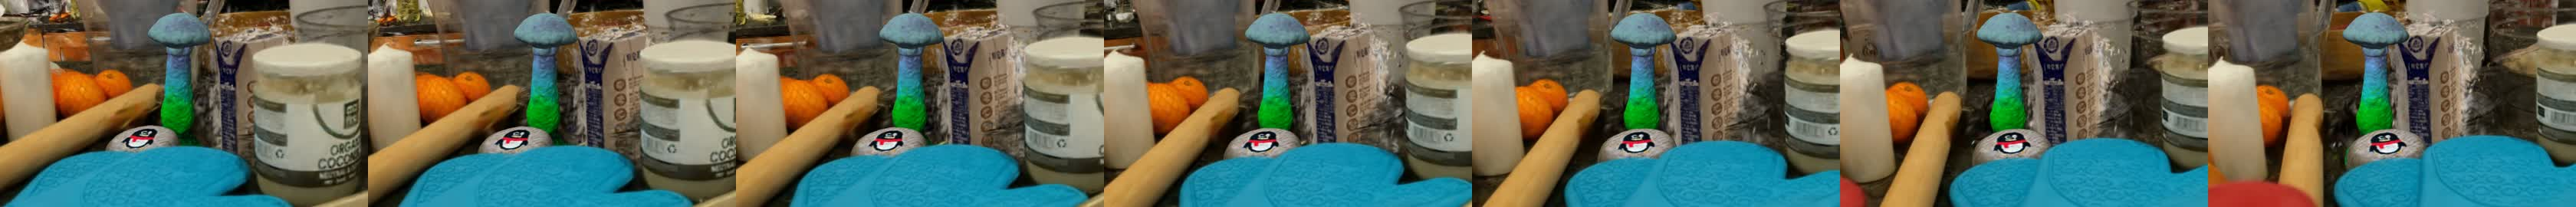
\includegraphics[width=\linewidth]{task1_fused_contact.jpg}
\caption{Task 1 最终融合视频关键帧接触表。相机始终围绕 A/B/C 前景资产观察，而不是沿背景厨房大范围漂移。}
\label{fig:task1-contact}
\end{figure}

\begin{figure}[!htbp]
\centering
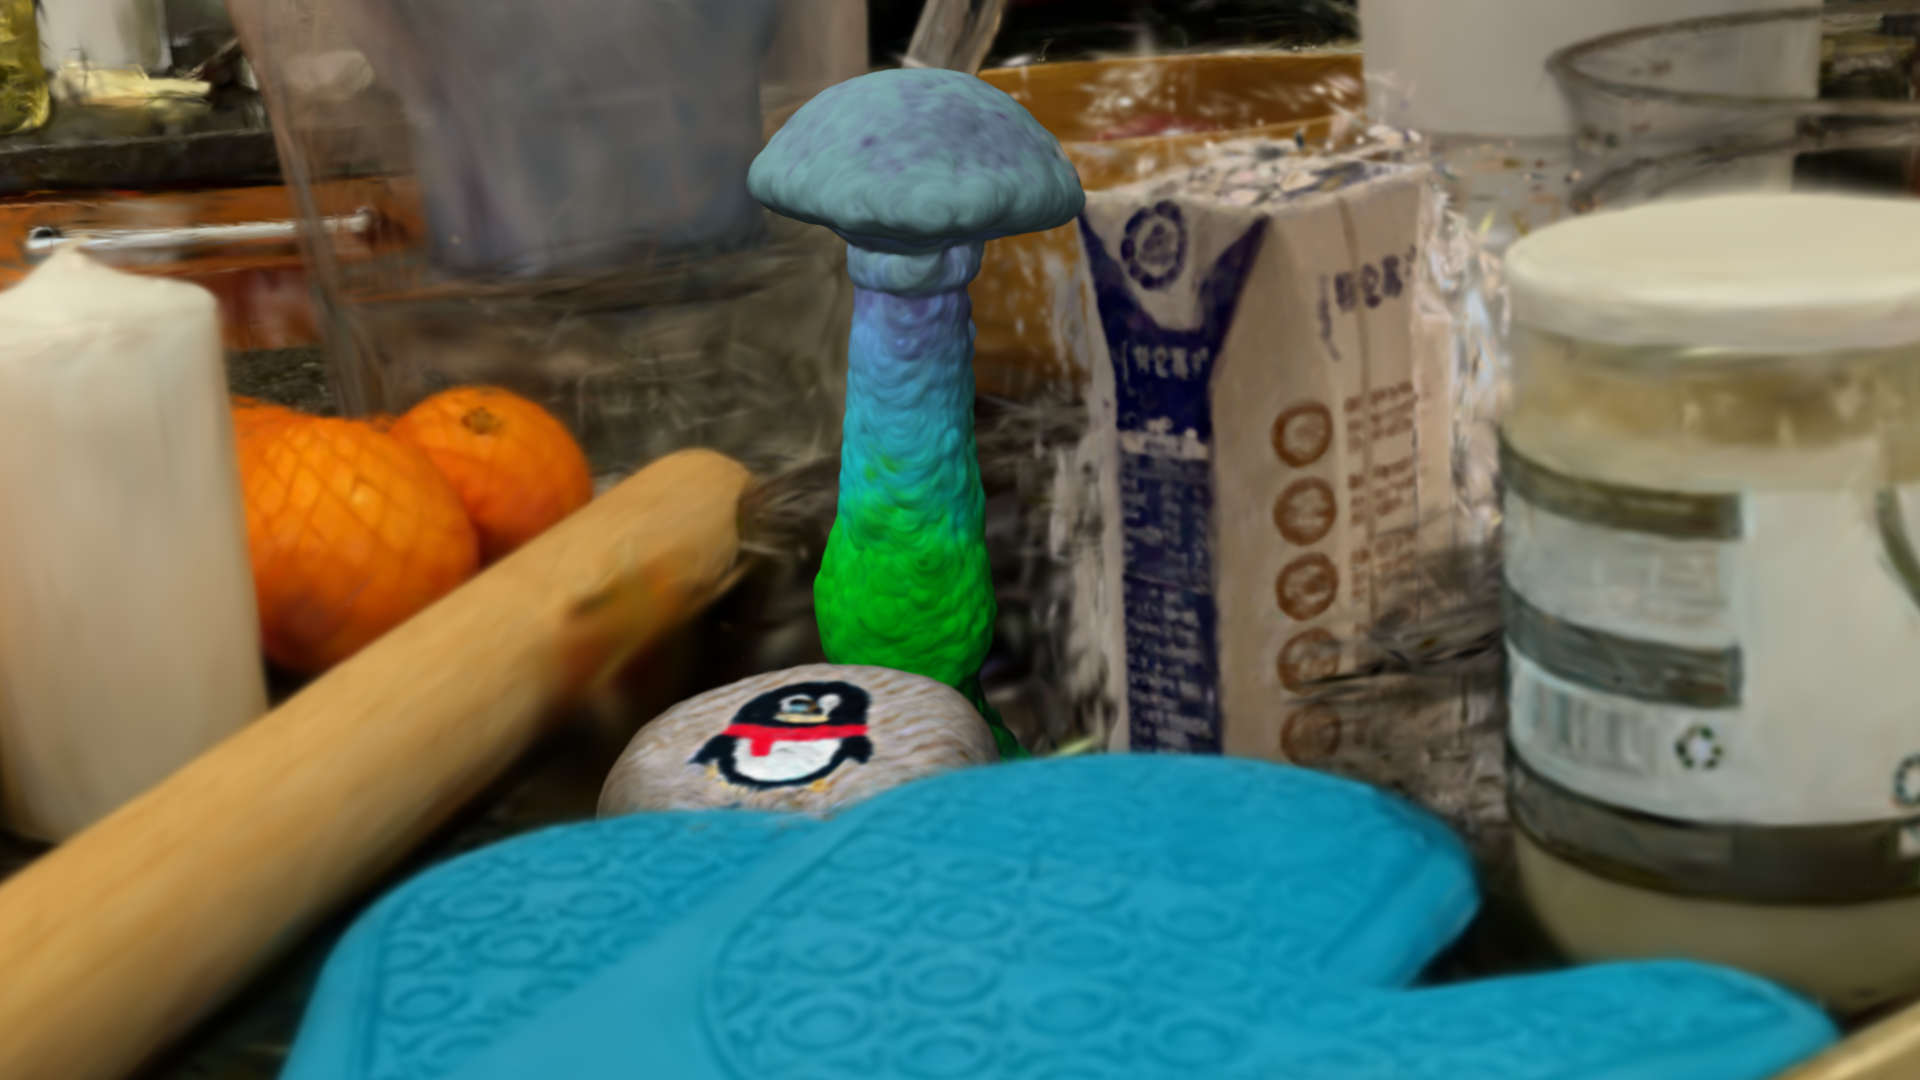
\includegraphics[width=0.82\linewidth]{task1_mid_frame.png}
\caption{Task 1 最终视频中间帧。A 为真实重建 splat，B/C 为 mesh surface splats，背景为 Mip-NeRF 360 counter 的 3DGS。}
\label{fig:task1-midframe}
\end{figure}

\begin{table}[!htbp]
\centering
\small
\caption{Task 1 最终融合渲染 manifest 摘要}
\label{tab:task1-render}
\begin{tabular}{@{}L{0.30\linewidth}L{0.55\linewidth}@{}}
\toprule
项目 & 数值 / 设置 \\
\midrule
Renderer & \texttt{gsplat fused splat renderer}，\texttt{pipeline\_mode=fused\_splats} \\
输出规格 & 1920$\times$1080，24 fps，144 frames，6.0 s \\
相机 & 前景 orbit；radius 2.20，height 1.02，target z 0.34，focal scale 1.476 \\
背景 splats & 494,805 \\
物体 A splats & 42,924；空间主体过滤 + 16.96$^\circ$ PCA 旋正 + 高亮通道上限 0.84 \\
物体 B splats & 260,000，从 OBJ 纹理表面采样 \\
物体 C splats & 120,000，从 OBJ 纹理表面采样 \\
验证 & \texttt{evaluate.py --strict-real-outputs}: PASS；单元测试 30/30 通过 \\
\bottomrule
\end{tabular}
\end{table}

\subsection{三种资产生成方式对比与现象分析}

表 \ref{tab:task1-compare} 从几何准确度、纹理细节和资产生成耗时三个维度比较多视角重建、文本生成和单图生成。这里的耗时指资产生成或重建阶段，而不是最终融合视频渲染时间；最终 144 帧 1080p 视频渲染对三类资产共享同一 \texttt{gsplat} pipeline，manifest 记录为 58.98 s，更适合作为最终 renderer 性能信息。由于 Nerfstudio、threestudio 和 Zero123 的日志格式并不完全一致，表中同时保留训练 steps 和日志/文件时间口径。整体来看，真实多视角重建最适合保留已观测物体的真实材质，但依赖拍摄质量和 COLMAP 注册；文本到 3D 最自由，但和 prompt 的颜色/细节一致性最弱；单图到 3D 生成开销最低，但未观测侧面的幻觉最明显。

\begin{table}[!htbp]
\centering
\small
\caption{Task 1 三种 3D 资产生成方式对比}
\label{tab:task1-compare}
\begin{tabularx}{\linewidth}{@{}L{0.16\linewidth}XXX@{}}
\toprule
维度 & A：真实多视角 3DGS & B：文本到 3D / SDS & C：单图到 3D / Zero123 \\
\midrule
输入信息 & 真实视频多帧，具有多视角几何约束 & 单段 prompt，无真实几何观测 & 单张真实图，正面信息强、背面无观测 \\
几何准确度 & 已观测表面最可信；少纹理和反光区域会产生 splat 噪声 & 形体语义可用，但由 2D 先验驱动，局部几何可能漂移 & 正面较稳定，侧/背面依赖生成先验，闭合性有限 \\
纹理细节 & 来自真实拍摄，局部文字和材质可保留；受曝光和重建质量影响 & 风格化明显；本实验颜色偏蓝绿，与 violet prompt 有偏差 & 保留输入图主视觉，但多视角纹理连续性弱于 A \\
资产生成耗时 & COLMAP/前处理日志约 20 min；30k 3DGS steps 的训练目录文件时间约 8.3 min & 15k SDS steps；从 checkpoint 到 OBJ/texture 导出的文件时间约 33 min，单步开销较高 & 1200 Zero123 steps；checkpoint/log 文件时间约 12 min，相对最轻量 \\
适合用途 & 真实物体复现、需要报告中体现重建能力的资产 & 创造不存在的虚拟物体、补充语义多样性 & 从一张实拍图快速扩展 3D 展示资产 \\
\bottomrule
\end{tabularx}
\end{table}

最终版本的主要视觉问题来自真实数据和表示差异，而不是后期合成。A 的原始 3DGS 表面存在少量白色碎片，这是拍摄曝光、反光材质和 splat 训练共同导致的。我们通过提高 A 的 opacity quantile、取消额外不透明放大、空间主体过滤、PCA 竖直化和高亮通道压制将问题控制在可接受范围内，但如果完全消除白色碎片，需要重新拍摄更均匀的 A 多视角素材或重新训练 A。B/C 的 surface splats 让 mesh 可以进入统一 renderer，但仍不如原生 3DGS 那样具有视角相关外观。背景方面，\texttt{counter} 的台面区域遮挡较多；我们选择前景聚焦相机和局部背景清除来保证三个插入物体可见，这是展示目标和物理遮挡之间的折中。

\FloatBarrier

\section{Task 2：基于 LeRobot 的 ACT 策略跨环境泛化挑战}

\subsection{任务要求与直观解释}

Task 2 主要看一个问题：视觉-动作策略换到没见过的 CALVIN 环境后，动作还稳不稳。每个 episode 可以理解成一段机器人操作演示，输入是主视角图像、腕部视角图像和机器人状态，输出是下一步或未来一小段动作。这里训练两个策略：一个只用环境 A 的演示，另一个混合使用环境 A/B/C 的演示；最后都放到没有参与训练的环境 D 上测试。若 A/B/C 模型在 D 上的动作误差更低，说明它不只是记住了环境 A 的背景和摆放方式，而是学到了一些更接近任务本身的操作规律。

具体做法分三步：先只用环境 A 训练一版 ACT；再在同样网络结构和核心超参数下，用环境 A/B/C 训练第二版；最后固定到环境 D 做 zero-shot 离线评估。数据沿用课程提供的 CALVIN LeRobot 划分，split 映射为 \texttt{splitA=A}、\texttt{splitB=B}、\texttt{splitC=C}、\texttt{splitD=D}。

\subsection{数据集与实验划分}

数据集采用课程提供的 \texttt{xiaoma26/calvin-lerobot} 划分。每个 episode 以 LeRobot/parquet 格式存储，核心字段包括主视角 \texttt{image}、腕部视角 \texttt{wrist\_image}、机器人状态 \texttt{state}、动作 \texttt{actions}、时间戳和任务索引。表 \ref{tab:task2-data} 给出训练和评估使用的数据规模。

\begin{table}[!htbp]
\centering
\small
\caption{Task 2 CALVIN LeRobot 数据划分}
\label{tab:task2-data}
\begin{tabular}{@{}L{0.18\linewidth}L{0.20\linewidth}R{0.18\linewidth}R{0.18\linewidth}L{0.18\linewidth}@{}}
\toprule
Split & 对应环境 & Episode 数 & Frame 数 & 用途 \\
\midrule
\texttt{splitA} & A & 6089 & 366693 & 单环境训练；联合训练 \\
\texttt{splitB} & B & 6115 & 367096 & 联合训练 \\
\texttt{splitC} & C & 5666 & 337954 & 联合训练 \\
\texttt{splitD} & D & 5124 & 308918 & zero-shot 评估 \\
\bottomrule
\end{tabular}
\end{table}

\subsection{方法：ACT 与动作分块机制}

ACT 的核心思想是一次预测未来一段动作，而不是每一帧只预测一个动作。本实验设置 chunk size 为 16，即模型根据当前双视角图像和机器人状态，一次输出未来 16 步动作片段。这样做有两个好处：一是动作序列更平滑，短时视觉噪声不会立刻导致动作大幅跳变；二是模型能在训练时看到动作片段内部的局部结构，例如接近物体、抓取、移动和释放之间的连续关系。

本实验直接调用 LeRobot 的 \texttt{ACTPolicy}，结构包括双视角图像编码、机器人状态编码、Transformer decoder 和 VAE 风格的训练目标。动作误差使用 Action L1，即预测动作和数据集中专家动作之间的平均绝对差。训练目标为 Action L1 与 KL 正则的加权和，其中动作分块长度为 16，\texttt{kl\_weight=10.0}。在跨环境评估中，环境 D 的背景、物体布局和视觉风格相对训练环境发生变化，因此模型是否仍能输出接近专家的动作，是衡量泛化能力的关键。

\subsection{训练配置}

两个模型保持相同网络结构和核心超参数，只改变训练数据来源。训练过程使用 mixed precision 加速；loss、Action L1、学习率曲线和配置摘要均导出到 \path{hw3/task2/results/}，便于和最终图表对应。

\begin{table}[!htbp]
\centering
\small
\caption{Task 2 ACT 训练配置}
\label{tab:task2-config}
\begin{tabular}{@{}L{0.30\linewidth}L{0.56\linewidth}@{}}
\toprule
项目 & 配置 \\
\midrule
模型 & LeRobot \texttt{ACTPolicy}，双视角图像 + 机器人状态输入 \\
训练任务 & \texttt{act\_splitA}: \texttt{splitA}；\texttt{act\_splitABC}: \texttt{splitA+splitB+splitC} \\
评估任务 & 两个模型均在 \texttt{splitD} 上 zero-shot 离线评估 \\
图像尺寸 & $96\times96$ \\
动作维度 / 状态维度 & action dim 7 / state dim 15 \\
动作分块长度 & \texttt{chunk\_size=16} \\
Transformer 配置 & hidden dim 256，heads 4，layers 3，dropout 0.1 \\
训练目标 & Action L1 + VAE KL 项，\texttt{kl\_weight=10.0} \\
优化器参数 & learning rate $1\times10^{-4}$，weight decay $1\times10^{-4}$ \\
训练轮数与 batch size & 8 epochs，train batch size 128，eval batch size 256 \\
随机种子与加速 & seed 42，AMP 开启，num workers 8 \\
实验记录 & GitHub \texttt{hw3/task2/results/curves/} 与 \texttt{results/figures/} \\
模型托管 & \href{https://modelscope.cn/models/youngchen/CS60003/tree/master/hw3/task2}{\texttt{youngchen/CS60003/hw3/task2/}} \\
\bottomrule
\end{tabular}
\end{table}

\subsection{训练曲线与收敛对比}

图 \ref{fig:task2-curves} 展示了训练日志导出的训练和验证曲线。\texttt{act\_splitABC} 的训练数据约为 \texttt{act\_splitA} 的三倍，因此总训练 step 更多；两者都能稳定下降，说明相同 ACT 结构在单环境和多环境训练下都能有效拟合专家动作。从验证曲线看，多环境联合模型在 D 环境上的 Action L1 始终处于更低区间，说明加入 B/C 环境不是简单增加训练时长，而是让模型见到更多视觉背景和操作变化，从而减少对环境 A 外观的过拟合。

\begin{figure}[!htbp]
\centering
\begin{subfigure}{0.47\textwidth}
  \centering
  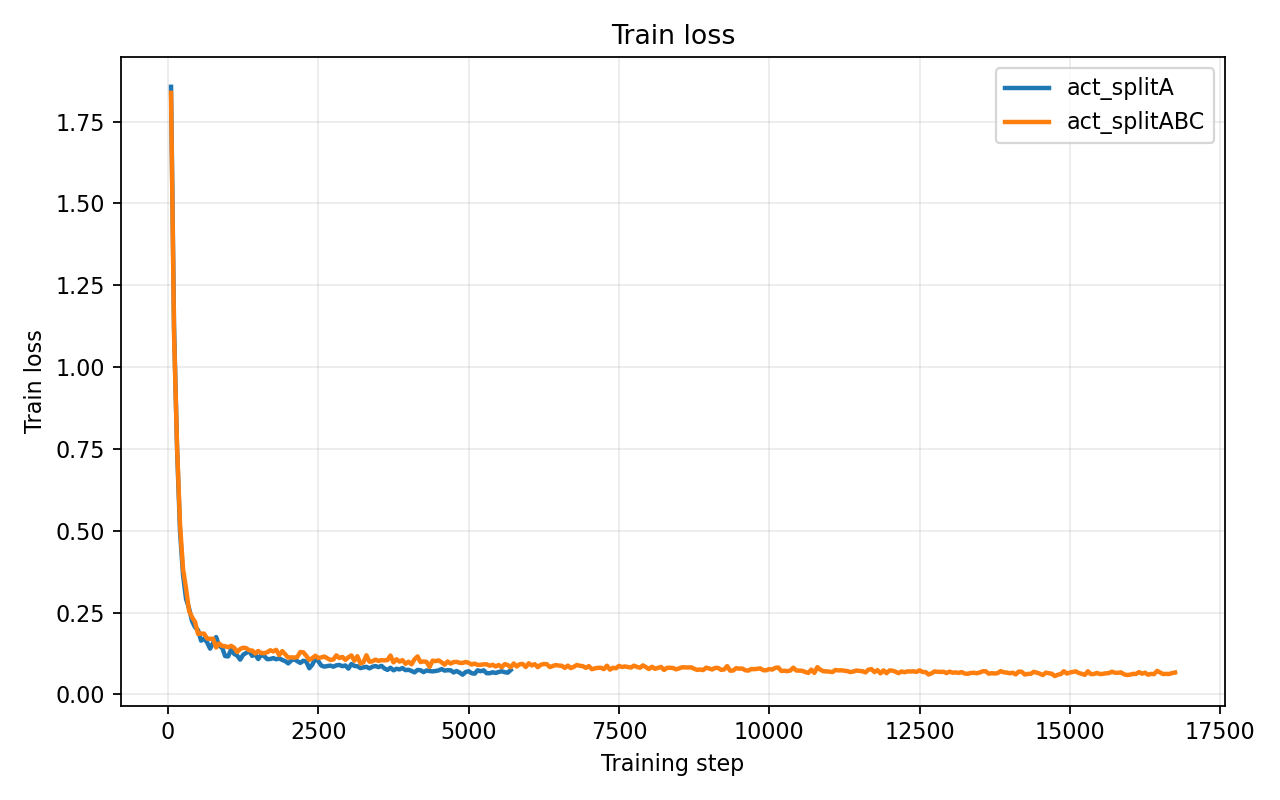
\includegraphics[width=\linewidth]{train_loss_curve.png}
  \caption{训练 loss 曲线}
\end{subfigure}\hfill
\begin{subfigure}{0.47\textwidth}
  \centering
  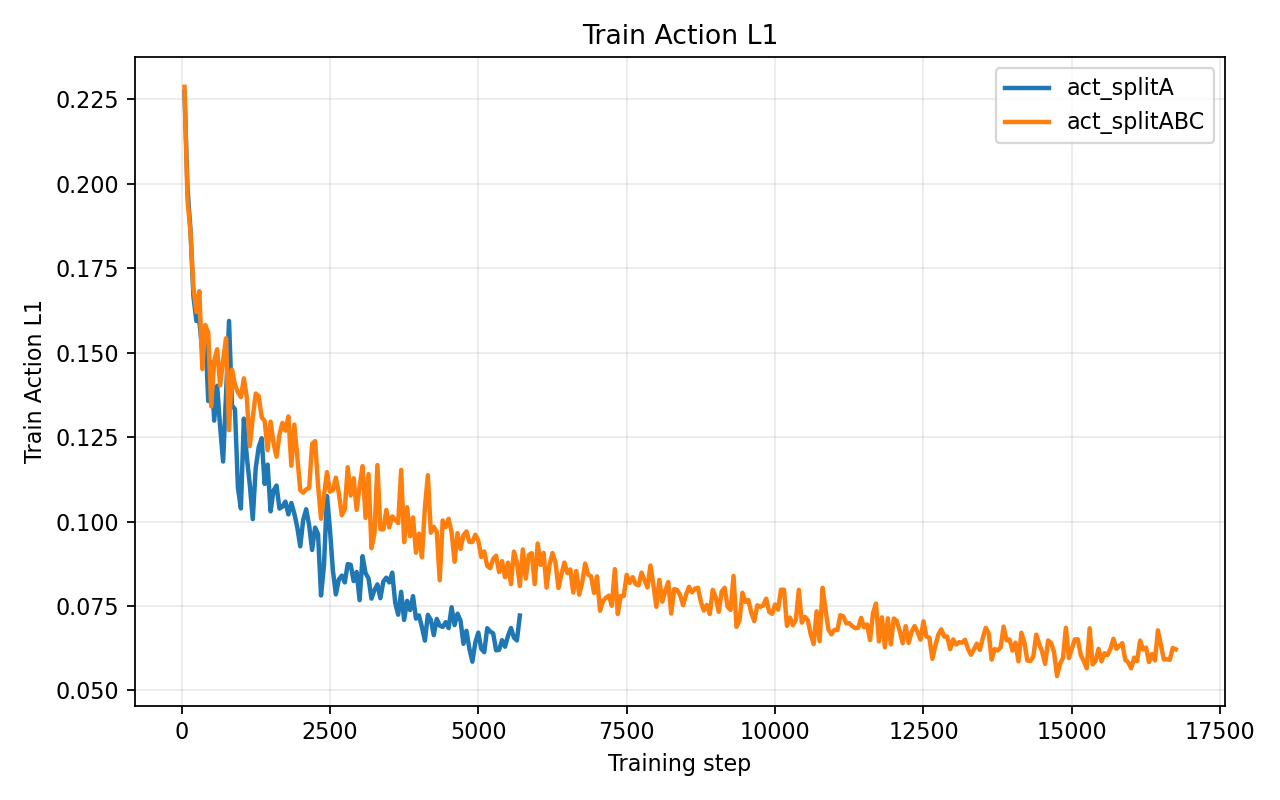
\includegraphics[width=\linewidth]{train_action_l1_curve.png}
  \caption{训练 Action L1 曲线}
\end{subfigure}
\vspace{6pt}

\begin{subfigure}{0.60\textwidth}
  \centering
  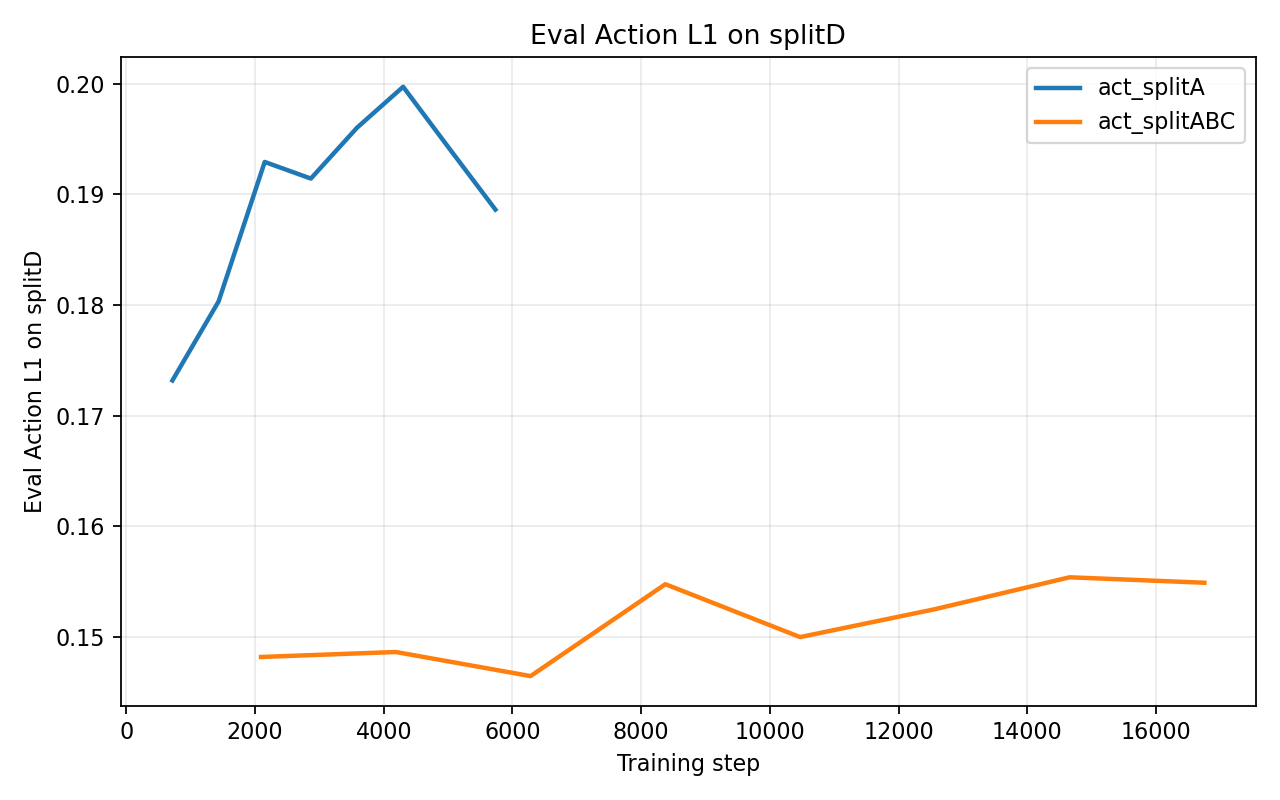
\includegraphics[width=\linewidth]{eval_action_l1_curve.png}
  \caption{环境 D 验证 Action L1 曲线}
\end{subfigure}
\caption{Task 2 训练曲线。源数据位于 GitHub 的 \texttt{hw3/task2/results/curves/}。}
\label{fig:task2-curves}
\end{figure}

\FloatBarrier

\subsection{Zero-shot 评估结果}

表 \ref{tab:task2-results} 汇总了两个模型在环境 D 上的 Action L1。主结论使用 \texttt{final.pt}，因为它没有根据 D 环境误差挑选 checkpoint，更接近真正的 zero-shot 评估。\texttt{act\_splitABC} 的 final Action L1 为 0.1549013643，低于 \texttt{act\_splitA} 的 0.1886211640，绝对下降 0.0337197997，相对提升 17.88\%。\texttt{best.pt} 结果也保持相同排序，但由于 best checkpoint 使用了 D 上离线误差做选择，因此只作为参考。

\begin{table}[!htbp]
\centering
\small
\caption{Task 2 环境 D zero-shot Action L1 结果}
\label{tab:task2-results}
\begin{tabularx}{\linewidth}{@{}lXrrr@{}}
\toprule
模型 & 训练数据 & {\texttt{final.pt} Action L1} & {\texttt{best.pt} Action L1} & 相对提升 \\
\midrule
\texttt{act\_splitA} & \texttt{splitA} & 0.1886211640 & 0.1731817282 & - \\
\texttt{act\_splitABC} & \texttt{splitA+splitB+splitC} & 0.1549013643 & 0.1464656246 & 17.88\% \\
\bottomrule
\end{tabularx}
\end{table}

\begin{figure}[!htbp]
\centering
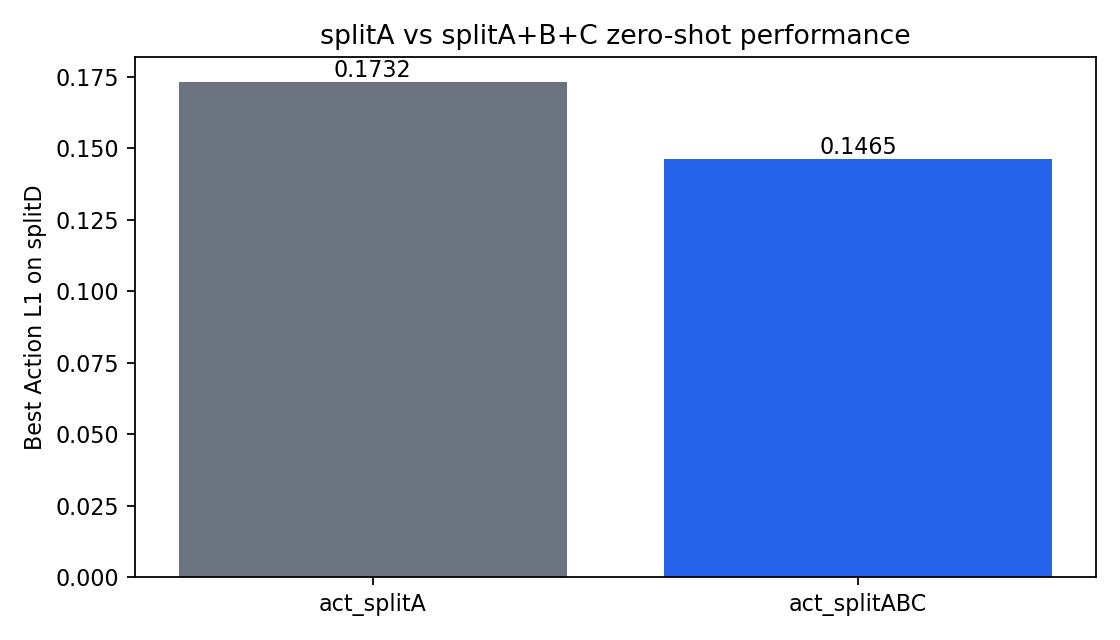
\includegraphics[width=0.88\textwidth]{splitA_vs_splitABC_eval_l1.png}
\caption{单环境训练与多环境联合训练在 splitD 上的 Action L1 对比。数值越低越好。}
\label{fig:task2-model-compare}
\end{figure}

\subsection{配对统计与稳定性分析}

仅看平均值可能掩盖局部失败，因此进一步按 episode、task 和动作维度做配对比较。表 \ref{tab:task2-stats} 显示，多环境模型不是只在少数样本上大幅改善，而是在大多数配对项上稳定更好：5124 个 episode 中有 4041 个更优，389 个任务索引中有 355 个更优，7 个动作维度全部更优。bootstrap 置信区间均为正，说明改进方向稳定。

\begin{table}[!htbp]
\centering
\small
\caption{Task 2 final checkpoint 配对统计摘要}
\label{tab:task2-stats}
\begin{tabularx}{\linewidth}{@{}lrrrrX@{}}
\toprule
粒度 & 配对数 & ABC 更优数 & ABC 更优比例 & 平均 L1 提升 & 95\% CI \\
\midrule
Episode & 5124 & 4041 & 78.86\% & 0.032959 & [0.031753, 0.034230] \\
Task & 389 & 355 & 91.26\% & 0.031384 & [0.028808, 0.034193] \\
Action dim & 7 & 7 & 100.00\% & 0.033752 & [0.012247, 0.070059] \\
\bottomrule
\end{tabularx}
\end{table}

这些统计让结论更稳。A-only 模型只见过一种背景和物体布局，更容易把特定视觉纹理和动作绑定在一起；A/B/C 联合模型见过同类任务在不同外观下的变化，更容易关注双视角图像里真正和操作有关的部分，例如机械臂、目标物体和接触状态。ACT 的动作分块也有帮助：模型预测的是一段动作，而不是单步反应，所以短时视觉偏移或局部遮挡不容易立刻把动作带偏。

\subsection{复现、托管与当前限制}

复现检查脚本位于 \path{hw3/task2/scripts/}，文件名为 \texttt{check\_reproducibility.sh}。它会检查四个 split 的 episode/frame 数、结果文件完整性，以及 \texttt{final.pt} 口径下 \texttt{act\_splitABC} 是否优于 \texttt{act\_splitA}。训练权重上传到 ModelScope 统一项目的 \href{https://modelscope.cn/models/youngchen/CS60003/tree/master/hw3/task2}{\texttt{youngchen/CS60003/hw3/task2/}} 子目录，包括两个模型的 \texttt{best.pt}、\texttt{final.pt}、\texttt{latest.pt}、配置、训练摘要和评估结果表。

需要说明的是，本文没有报告官方 CALVIN simulator 的真实 Success Rate，而是采用任务允许的动作误差作为 zero-shot 指标。原因是当前 LeRobot splitD 缺少官方 simulator 评估所需的原始 \path{validation/.hydra/merged_config.yaml}，直接运行官方 Success Rate 脚本会缺少环境状态配置。相关探测只保留在交付目录的脚本和日志中；就这份报告而言，Action L1 是更可复现、也更适合横向比较的主指标。

\section{结论}

Task 1 实现了完整的多源 3D 资产融合链路：真实物体 A 使用 COLMAP + 3DGS，虚拟物体 B 使用文本到 3D/SDS，真实单图物体 C 使用 Zero123，背景使用 Mip-NeRF 360 \texttt{counter} 的 3DGS。最终没有采用 2D 后合成，而是把 A/background 的 splat 与 B/C 的 mesh surface splats 统一到同一个 \texttt{gsplat} renderer 中，并通过前景聚焦相机生成 1080p 多视角视频。实验也显示三种资产路径各有取舍：多视角重建真实性最好但依赖拍摄和 COLMAP；文本生成自由度高但 prompt 一致性有限；单图生成开销较低但背面/侧面更依赖先验。

Task 2 给出了 ACT 跨环境泛化实验：\texttt{act\_splitA} 使用环境 A 训练，\texttt{act\_splitABC} 使用环境 A/B/C 联合训练，两个模型都在未见过的环境 D 上评估。按 \texttt{final.pt} 计算，联合训练将 Action L1 从 0.1886211640 降至 0.1549013643，相对提升 17.88\%；episode、task 和动作维度的配对统计也一致支持该结论。整体来看，多环境数据提升了 ACT 策略对视觉分布偏移的鲁棒性，动作分块机制则帮助策略在短时视觉变化下保持更平滑、更稳定的动作输出。

\end{document}
